\section{LEVEL 1 · Statistisch onderzoek}

\begin{missie}
Missie: ontdek hoe een statistisch onderzoek stap voor stap verloopt.
\end{missie}

\begin{doel}
\textbf{DOEL} \quad Na dit level kan je:

☐ uitleggen wat statistiek is en de \textbf{stappen van een onderzoek} in de juiste volgorde zetten;

☐ een \textbf{probleemstelling}, een \textbf{onderzoeksvraag} en een \textbf{hypothese} onderscheiden;

☐ een \textbf{variabele} benoemen en bepalen of ze \textbf{kwantitatief} of \textbf{kwalitatief} is;

☐ het \textbf{soort data} bepalen (numeriek, categorisch geordend, categorisch niet-geordend).
\end{doel}

\subsection*{Theorie 1.1 · Wat is statistiek? De onderzoekscyclus}

\begin{theorie}
\textbf{Statistiek} is de wetenschap die zich bezighoudt met het \textbf{verzamelen}, \textbf{verwerken}, \textbf{analyseren} en \textbf{interpreteren} van gegevens of \textbf{data}. Het doel van statistiek is informatie halen uit data.

Een statistisch onderzoek verloopt in \textbf{acht stadia}. Na stap 8 kan een nieuwe onderzoeksvraag ontstaan en begint de cyclus opnieuw.
\end{theorie}

\begin{center}
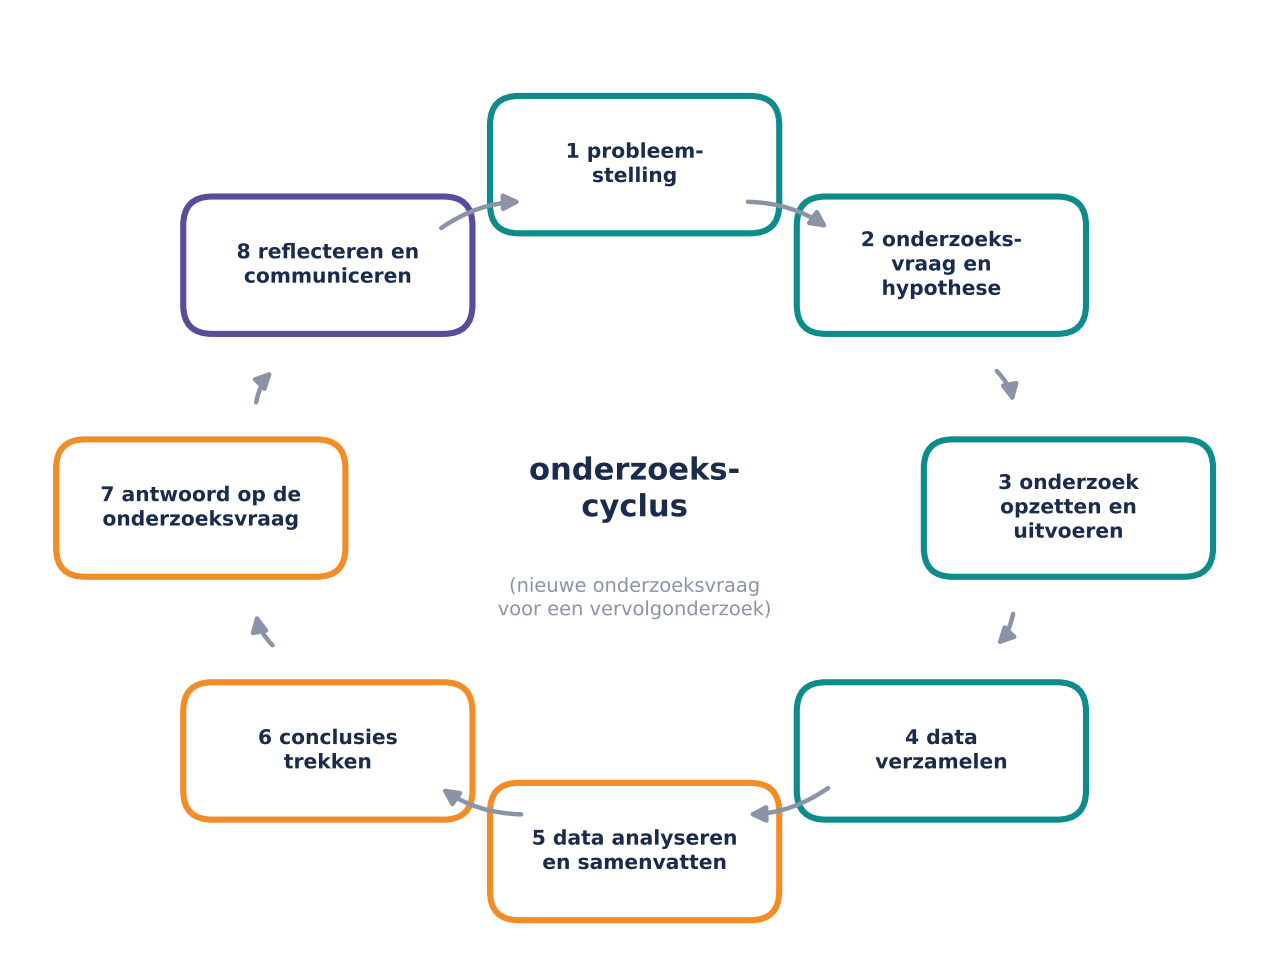
\includegraphics[width=0.8\textwidth]{figuren/d1_cyclus.png}
\end{center}

\begin{voorbeeld}
\textbf{Voorbeeld.} Een kinderopvang merkt dat veel ouders hun kind te laat komen halen.

\breedtes{34/66}
\begin{tabular}{ll}
\hline
Stap & In het voorbeeld \\
\hline
1 probleemstelling & Veel ouders komen hun kind na sluitingstijd halen. \\
2 onderzoeksvraag en hypothese & Vraag: ‘Hoe laat komen de ouders hun kind gemiddeld halen?’ Hypothese: ‘Minstens de helft komt na 17.30 uur.’ \\
3 onderzoek opzetten en uitvoeren & Een korte vragenlijst opstellen en plannen. \\
4 data verzamelen & De ouders vullen de vragenlijst in. \\
5 data analyseren en samenvatten & Tabellen, grafieken en gemiddelden maken. \\
6 conclusies trekken & De resultaten bekijken en interpreteren. \\
7 antwoord op de onderzoeksvraag & ‘Gemiddeld komt men om 17.40 uur.’ \\
8 reflecteren en communiceren & Het resultaat aan de ouders meedelen en de openingsuren bespreken. \\
\hline
\end{tabular}
\end{voorbeeld}

\subsection*{Theorie 1.2 · Variabelen en soorten data}

\begin{theorie}
Een \textbf{variabele} is een kenmerk dat we willen onderzoeken bij een groep personen of voorwerpen. Alle gegevens samen vormen de \textbf{dataset}.

\begin{itemize}
\item Bij een \textbf{kwantitatieve} variabele zijn de data \textbf{numeriek}: je kan er zinvol mee rekenen (gemiddelde, histogram, boxplot).
\item Bij een \textbf{kwalitatieve} variabele zijn de data \textbf{categorisch}. Die kunnen \textbf{geordend} zijn (er is een volgorde) of \textbf{niet-geordend}.
\end{itemize}

\breedtes{30/30/40}
\begin{tabular}{lll}
\hline
Variabele & Soort & Voorbeeld van data \\
\hline
leeftijd van een bewoner & kwantitatief, numeriek & 71, 96, 84, 101, 83 \\
tevredenheid van een ouder & kwalitatief, categorisch geordend & zeer ontevreden, ontevreden, neutraal, tevreden, zeer tevreden \\
burgerlijke staat van een collega & kwalitatief, categorisch niet-geordend & ongehuwd, samenwonend, gehuwd \\
postcode van een kind & kwalitatief, categorisch niet-geordend & 9000, 9050, 9040 \\
\hline
\end{tabular}
\end{theorie}

\begin{letop}
\textbf{LET OP} \quad Een postcode bestaat uit cijfers maar is een \emph{label}: de data zijn categorisch. Je kan geen zinvol gemiddelde van postcodes berekenen.
\end{letop}

\subsection*{Aan de slag}

\subsubsection*{Oefening 1.1 \quad ★☆☆ \quad Invullen: de onderzoekscyclus}

\textbf{Woordenlijst:} onderzoeksvraag – hypothese – probleemstelling – data – conclusies – communiceren.

Een onderzoek start met een \gat{probleemstelling}. Daaruit formuleer je een \gat{onderzoeksvraag} en een \gat{hypothese}, een veronderstelling over het antwoord. Daarna verzamel je \gat{data}, analyseer je ze en trek je \gat{conclusies}. Op het einde reflecteer je en ga je \gat{communiceren} over de resultaten.

\subsubsection*{Oefening 1.2 \quad ★★☆ \quad Zet de stappen in de juiste volgorde}

De leiding van een jeugdbeweging onderzoekt welke kampbestemming de leden verkiezen. Zet de activiteiten in de juiste volgorde.

\textbf{A} De leiding besluit dat ‘strand’ de populairste bestemming is en bespreekt dat met de leden.

\textbf{B} De leiding merkt dat de leden het moeilijk eens raken over de kampbestemming.

\textbf{C} De antwoorden worden in Excel ingevoerd en in tabellen en grafieken verwerkt.

\textbf{D} De leiding formuleert de onderzoeksvraag ‘Welke kampbestemming verkiezen de leden?’ en veronderstelt dat de meeste leden voor het strand kiezen.

\textbf{E} De vragenlijst wordt rondgestuurd en door de leden ingevuld.

\textbf{F} De leiding stelt een vragenlijst op.

\textbf{G} De resultaten verschijnen in de nieuwsbrief en men overweegt het volgend jaar opnieuw te bevragen.

De juiste volgorde: \_\_ – \_\_ – \_\_ – \_\_ – \_\_ – \_\_ – \_\_

\begin{oplossing}
\textbf{Oplossing 1.2} \quad B – D – F – E – C – A – G (probleemstelling, onderzoeksvraag en hypothese, opzetten, verzamelen, analyseren, conclusie, communiceren).
\end{oplossing}

\subsubsection*{Oefening 1.3 \quad ★★☆ \quad Context: vragen en variabelen}

Een woonzorgcentrum bevraagt zijn bewoners. Noteer bij elke vraag de onderzochte variabele en zet een kruisje als de variabele kwantitatief is.

\breedtes{44/38/18}
\begin{tabular}{lll}
\hline
Enquêtevraag & Variabele & Kwantitatief? \\
\hline
1. Hoeveel keer per week krijg je bezoek? & & \\
2. Hoe tevreden ben je over de maaltijden? (zeer ontevreden – ontevreden – neutraal – tevreden – zeer tevreden) & & \\
3. Welke activiteit doe je het liefst? (kaarten, wandelen, knutselen, zingen) & & \\
4. Hoeveel minuten wacht je gemiddeld op hulp nadat je op de bel drukte? & & \\
\hline
\end{tabular}

Noteer ook bij vraag 2 en 3 het soort data. \lijn

\begin{oplossing}
\textbf{Oplossing 1.3} \quad 1. het aantal bezoeken per week – kwantitatief (x). 2. de tevredenheid over de maaltijden – niet kwantitatief; categorisch geordend. 3. de favoriete activiteit – niet kwantitatief; categorisch niet-geordend. 4. de wachttijd (in minuten) op hulp – kwantitatief (x).
\end{oplossing}

\subsubsection*{Oefening 1.4 \quad ★★☆ \quad Waar of vals?}

Is de bewering altijd waar? Verklaar.

\textbf{a)} Van een kwantitatieve variabele kan je steeds een rekenkundig gemiddelde berekenen. \lijn

\textbf{b)} Bij een kwalitatieve variabele is het onmogelijk om een modus te bepalen. \lijn

\textbf{c)} Data van een kwantitatieve variabele kan je soms voorstellen met een histogram. \lijn

\textbf{d)} Data van een kwalitatieve variabele kan je voorstellen met een boxplot. \lijn

\begin{oplossing}
\textbf{Oplossing 1.4}

a) Waar: bij een kwantitatieve variabele zijn de data numeriek en met numerieke data kan je rekenen. b) Vals: bij categorische data kan je vaak wel de modus (meest voorkomende categorie) bepalen. c) Waar: numerieke data kan je in veel gevallen samenvatten in een histogram. d) Vals: een boxplot vraagt numerieke data (mediaan en kwartielen).
\end{oplossing}

\subsubsection*{Oefening 1.5 \quad ★★★ \quad Een eigen onderzoek starten}

Een buitenschoolse opvang vermoedt dat kinderen na een sportnamiddag beter slapen. Werk de eerste stappen uit.

\textbf{a)} Formuleer een probleemstelling, een onderzoeksvraag en een hypothese. \lijn

\textbf{b)} Welke variabele(n) onderzoek je? Is die kwantitatief of kwalitatief? \lijn

\textbf{c)} Hoe zou je de data verzamelen en hoe zou je ze verwerken (stappen 3 – 5)? \lijn

\begin{oplossing}
\textbf{Oplossing 1.5} \quad (Meerdere antwoorden mogelijk.) a) Probleem: sommige kinderen slapen ’s avonds moeilijk in. Onderzoeksvraag: ‘Slapen kinderen beter na een sportnamiddag?’ Hypothese: ‘Kinderen slapen na een sportnamiddag gemiddeld langer.’ b) Het aantal uur slaap (kwantitatief), eventueel ‘heeft sportnamiddag gehad ja/nee’ (kwalitatief). c) Een korte vragenlijst voor de ouders of een slaaplogboek; de data in Excel invoeren en gemiddelden en grafieken per groep maken.
\end{oplossing}

\subsection*{Koppel · begrip en voorbeeld}

Koppel elk begrip aan het juiste voorbeeld.

\breedtes{34/66}
\begin{tabular}{ll}
\hline
Begrip & Voorbeeld \\
\hline
1. probleemstelling & A. ‘Kinderen die sporten slapen gemiddeld langer.’ \\
2. hypothese & B. De ouders vullen het slaaplogboek een week in. \\
3. data verzamelen & C. ‘Sommige kinderen slapen moeilijk in.’ \\
4. kwantitatieve variabele & D. de tevredenheid over de maaltijd \\
5. categorisch geordende data & E. het aantal uur slaap per nacht \\
\hline
\end{tabular}

Mijn antwoord: 1 – \_\_\quad 2 – \_\_\quad 3 – \_\_\quad 4 – \_\_\quad 5 – \_\_

\begin{oplossing}
\textbf{Oplossing Koppel} \quad 1 – C \quad 2 – A \quad 3 – B \quad 4 – E \quad 5 – D
\end{oplossing}

\subsection*{CHECK · Level 1}

\textbf{1.} (2 p) Wat is statistiek? Noem twee dingen die je met data doet. \lijn

\textbf{2.} (2 p) Wat is het verschil tussen een onderzoeksvraag en een hypothese? \lijn

\textbf{3.} (2 p) Is ‘het aantal broers en zussen’ kwantitatief of kwalitatief? Welk soort data zijn dat? \lijn

\textbf{4.} (2 p) Waarom is een gemiddelde van postcodes zinloos? \lijn

\begin{doel}
\textbf{Score:} \_\_\_ / 8 \quad ☐ behaald (vanaf 5 / 8) \quad ☐ nog even oefenen
\end{doel}

\begin{oplossing}
\textbf{Oplossing CHECK 1}

1. Statistiek is de wetenschap van het verzamelen, verwerken, analyseren en interpreteren van data. 2. De onderzoeksvraag is de vraag die je wil beantwoorden; de hypothese is je veronderstelling over het antwoord. 3. Kwantitatief; numerieke data (discreet). 4. Een postcode is een label (categorisch), geen hoeveelheid; rekenen heeft geen betekenis.
\end{oplossing}
